\begin{figure}[H]
    \centering
    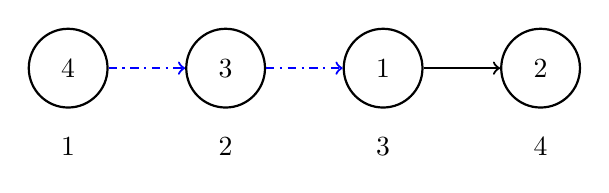
\begin{tikzpicture}[thick]
        \edef\pos{0}
        \foreach \x in {1, 2,..., 4}{
            \pgfmathparse{\pos+2}
            \xdef\pos{\pgfmathresult}
            \node  at (\pos, -1) {$\x$};
        }
        \node[circle,draw, minimum size=1cm] (1) at  (2, 0) {$4$};
        \node[circle,draw, minimum size=1cm] (2) at  (4, 0) {$3$};
        \node[circle,draw, minimum size=1cm] (3) at  (6, 0) {$1$};
        \node[circle,draw, minimum size=1cm] (4) at  (8, 0) {$2$};
        \draw[->, color=blue, dashdotted] (1) -- (2);
        \draw[->, color=blue, dashdotted] (2) -- (3);
        \draw[->] (3) -- (4);
        % \draw[->] (1) edge (2) (2) edge (3) (3) edge (4) (4) edge (5)
    \end{tikzpicture}
    \caption[Certificados atualizados]{Após a mudança de velocidade, no instante $t = 2.1$,
        do elemento 3, que se encontra em \sorted[2], \cert[1] e
        \cert[2] foram atualizados.}
    \label{fig:lista:after}
\end{figure}